\chapter{El caso finito}
\noindent
Nuevamente inspirados por el teorema \ref{theory:th:feasibility}, en este capítulo analizamos el
caso en el que el vector coprimo $\vec{q}$ tiene entradas estrictamente positivas. De esta manera,
el problema \eqref{theory:formulation} deviene una instancia particular del famoso Problema de la
Mochila:
\begin{subequations}
	\label{knapsack-formulation}
	\begin{align}
		\max_{\vec{x} \in \Z^n} \quad
			& \vec{u}^T\vec{x}, \\
		\text{s.a.} \quad
			& \vec{w}^T\vec{x} \leq c, \\
			& \vec{x} \geq \vec{0},
	\end{align}
\end{subequations}
donde los vectores positivos $\vec{u}, \vec{w} \in \Z^n$ son conocidos como vector de útiles y
vector de pesos, respectivamente. Puesto que no acotamos $\vec{x}$, el problema recibe el nombre de
Problema de la Mochila no Acotado. Pero también como $\vec{u} = \vec{w}$, el problema puede
ser considerado como un Problema de la Suma de Conjuntos no Acotado.

En la primera sección realizamos un análisis de capas enteras a fin de obtener un resultado análogo
al teorema \ref{infinite:th:complexity}. En concreto, el teorema \ref{th:intnonneg2} enuncia que,
para un presupuesto $u$ suficientemente grande en el problema \eqref{theory:formulation}, la
búsqueda de una solución se reduce a resolver solamente una ecuación lineal diofantina.

El resultado anterior, si bien interesante, es de existencia y no muestra cómo obtener las
soluciones enteras no negativas de ecuaciones lineales diofantinas. De manera similar a como lo
hicimos en el capítulo anterior, la segunda sección se encarga de presentar tal construcción de
soluciones a partir de los Algoritmos \ref{algo:fin:helper} y \ref{algo:fin:dioph}.

Finalmente, en la tercera y última sección de este capítulo, realizamos algunos experimentos
numéricos que comparan la eficacia de nuestros algoritmos recién desarrollados con la de
Ramificación y Acotamiento, así como de una formulación alternativa de programación dinámica.

\section{Análisis de capas enteras}
\noindent
De acuerdo al segundo caso del teorema \ref{theory:th:feasibility}, el número de puntos enteros no
negativos sobre la $k$-ésima capa entera es finito y, por lo tanto, puede ser cero. Sea $k \in
\braces{\eta, \ldots, 0}$. Sabemos de la Sección \ref{subsec:dioph-eq} que deseamos resolver la
ecuación lineal diofantina \eqref{eq:dioph}, por lo que implementamos la misma estrategia para
plantear una formulación recursiva. 

Debido al supuesto $\vec{q} > \vec{0}$, observemos de \eqref{dummy:eq:ith-equation} que podemos
agregar la condición $\omega_{i} \geq 0$. En efecto, buscamos que $\vec{x}$ sea no negativo y
recordemos que $g_i$ es un máximo común divisor (ver \eqref{dummy:eq:ith-g}), por lo que es
estrictamente positivo. Juntando esto con el supuesto $\vec{q} > \vec{0}$, encontramos que
$\omega_i$ es no negativo para toda $i \in \braces{1, \ldots, n - 1}$. Así pues, despejando $t_i$ de
\eqref{eq:recurrence} obtenemos los intervalos de factibilidad
\begin{equation*}
	\label{phase-1:finite:eq:param-bounds}
	\left\lceil -\frac{\omega_ix_i'}{g_{i+1}} \right\rceil
	\leq
	t_i
	\leq
	\left\lfloor \frac{\omega_i\omega_{i+1}'}{q_i} \prod_{j=1}^{i}g_j \right\rceil,
\end{equation*}
para todo $i \in \lbrace 1, \ldots, n - 2\rbrace$. Luego, como $0 < q_{n - 1}, q_n$, se sigue de
\eqref{eq:last-solution} que
\begin{equation*}
	\label{phase-1:finite:eq:param-bounds-last}
	\left\lceil -\frac{\omega_{n-1}x_{n-1}'}{q_n} \cdot \prod_{j=1}^{n-2}g_j \right\rceil
	\leq
	t_{n - 1}
	\leq
	\left\lfloor \frac{\omega_{n-1}x_{n}'}{q_{n-1}} \cdot \prod_{j=1}^{n-2}g_j \right\rfloor.
\end{equation*}

Consecuentemente, el número de elecciones que podemos realizar para el vector de variables libres
$\vec{t} \in \Z^{n-1}$ es, como lo confirma el teorema \ref{theory:th:feasibility}, finito. Si
determinamos que no existe tal punto en la $k$-ésima capa entera, descendemos a la $(k -1)$-ésima
capa entera y continuamos con nuestra búsqueda.

% Observemos también que una elección de $t_i$ modifica $\omega_{i+1}$ y por lo tanto también afecta
% el intervalo de factibilidad de $t_{i+1}$. Siguiendo con este razonamiento, encontramos que una
% elección de $t_i$ afecta a su vez los intervalos de factibilidad de $t_{i+1}, \ldots, t_{n-1}$. En
% la Sección \ref{subsec:complex} discutiremos cómo es que esta ``cadena'' acota la complejidad
% algorítmica del Algoritmo \ref{algo:fin:dioph}.

Ahora bien, en esta primera parte de la sección nos encargamos de calcular una cota superior para el
número de capas enteras que debemos analizar de manera que garanticemos la existencia de un punto
entero no negativo sobre una de estas capas enteras.

% En la primera parte de esta sección determinamos una cota superior para el número de capas enteras
% que visitamos y analizamos el comportamiento a medida que el presupuesto $u$ aumenta. En la segunda
% parte de esta sección mostramos que si el presupuesto $u$ es suficientemente grande, entonces la
% solución de (\ref{theory:formulation}) sí se encuentra sobre la $\eta$-ésima capa entera. Este
% resultado es análogo al caso infinito del teorema \ref{theory:th:feasibility}. Finalmente, en la
% tercera parte de esta sección discutimos brevemente sobre la complejidad algorítmica de encontrar
% la solución.

\begin{lemma}
	\label{lemma:tau}
	Sea $\vec{p} \in \R^n$ un vector esencialmente entero y sea $\vec{q} \in \Z^n$ su múltiplo
	coprimo, por lo que existe $m \in \R$ tal que $\vec{p} = m\vec{q}$. Supongamos que $m > 0$ y que
	$\vec{q} > \vec{0}$. Sea $q^* \coloneq \max\lbrace q_1, \ldots, q_n \rbrace$, y sea
	\begin{equation}
		\label{eq:tau}
		\tau \coloneq \left\lfloor \left\lfloor \frac{u}{q^*} \right\rfloor
			\frac{q^*}{m} \right\rfloor,
	\end{equation}
	donde $u$ es el lado derecho de \eqref{theory:constraint:budget}. Entonces la solución del
	problema \eqref{theory:formulation}, de ser factible, se encuentra en una capa entera
	parametrizada por $k \in \lbrace \eta, \eta - 1, \ldots, \tau \rbrace$, donde recuperamos $\eta$
	del lema \ref{phase-1:lemma:eta}.
\end{lemma}
\begin{proof}
	Definamos $i^* \coloneq \argmax\braces{q_1, \ldots, q_n}$ y consideremos el vector
	\begin{equation*}
		\vec{v} \coloneq \left\lfloor \frac{u}{q^*} \right\rfloor \vec{e}_{i^*}.
	\end{equation*}
	Por hipótesis tenemos $q^* > 0$ y, además, como el problema
	\eqref{theory:formulation} es factible, se sigue del teorema \ref{theory:th:feasibility} que el
	presupuesto $u$ es no negativo. De esto obtenemos que $\vec{v} \geq \vec{0}$. Así también,
	\begin{equation*}
		\vec{q}^T\vec{v} = \left\lfloor \frac{u}{q^*} \right\rfloor q^*
		\leq \frac{u}{q^*}q^* = u,
	\end{equation*}
	y entonces $\vec{v}$ es factible. De aquí se sigue que este vector provee una cota inferior para
	el problema (\ref{theory:formulation}). Así pues, todo vector $\vec{x}$ candidato a ser el
	óptimo del problema satisface
	\begin{equation*}
		\vec{q}^T\vec{x} = \frac{\vec{p}^T\vec{x}}{m} \geq \frac{\vec{q}^T\vec{v}}{m} = 
		\floor{\frac{u}{q^*}} \frac{q^*}{m}.
	\end{equation*}
	Nos interesa determinar el entero $\tau$ más pequeño tal que todo punto sobre la capa
	entera $H_{\vec{q}, k\norm{\vec{q}}^{-2}}$ con $k \in \lbrace \tau, \tau + 1, \ldots \rbrace$
	satisfaga esta desigualdad. Del lema \ref{phase-1:lemma:layer}, encontramos que $k$ debe satisfacer
	\begin{equation*}
		\frac{k}{\norm{\vec{q}}^{2}} = \frac{\vec{q}^T\vec{x}}{\norm{\vec{q}}^2} \geq
		\left\lfloor \frac{u}{q^*} \right\rfloor \frac{q^*}{m}
		\frac{1}{\norm{\vec{q}}^2},
	\end{equation*}
	equivalentemente,
	\begin{equation*}
		k \geq \floor{\frac{u}{q^*}}\frac{q^*}{m}.
	\end{equation*}
	Consecuentemente,
	\begin{equation*}
		\tau =
		\left\lfloor \left\lfloor \frac{u}{q^*} \right\rfloor \frac{q^*}{m}
			\right\rfloor.
	\end{equation*}
	Finalmente, recordemos del lema \ref{phase-1:lemma:eta} que $\eta$ es la primera capa en
	satisfacer la restricción presupuestaria. Por lo tanto, el óptimo del problema
	\eqref{theory:formulation} se encuentra en una capa entera parametrizada por $\tau \leq k \leq \eta$.
\end{proof}

\begin{observation}
	Siempre se cumple que $\tau \leq \eta$. En efecto,
	\begin{equation*}
		\left\lfloor \frac{u}{q^*} \right\rfloor q^*
		\leq \frac{u}{q^*} q^* = u,
	\end{equation*}
	como $m > 0$, tenemos
	\begin{equation*}
		\left\lfloor \frac{u}{q^*} \right\rfloor \frac{q^*}{m}
		\leq \frac{u}{m}.
	\end{equation*}
	Aplicando la función piso a ambos lados de la desigualdad y comparando con \eqref{eq:tau} y el
	lema \ref{phase-1:lemma:eta} encontramos que $\tau \leq \eta$.
\end{observation}
\begin{observation}
	Nuevamente, la suposición de que el escalar $m$ sea positivo ocurre sin pérdida de generalidad.
	Así como mencionamos en el capítulo anterior que si $m$ es negativo entonces existe un parámetro
	$\eta'$ análogo a $\eta$, también existe $\tau' \geq \eta'$ tal que la solución del problema
	\eqref{theory:formulation} se encuentra en una capa parametrizada por $\eta' \leq k \leq \tau'$.
\end{observation}


% Es decir, a pesar de que el óptimo se encuentre sobre la capa entera $k$ que estamos analizando, la
% elección de los primeros parámetros que realicemos puede afectar el tiempo de terminación de nuestro
% algoritmo. Hay dos extremos en las posibles estrategias que podemos adoptar para realizar estas
% elecciones. Para visualizarlo, tenemos que nuestro presupuesto actual $\omega_{i}$ determina el
% siguiente presupuesto a partir de
% \begin{equation*}
% 	\begin{cases}
% 		x_i = \omega_ix_i' + g_{i+1}t_i, \\
% 		\omega_{i+1} = \omega_i\omega_{i+1}' - \frac{q_i}{\prod_{j=1}^{i}g_j}t_i,
% 	\end{cases}
% \end{equation*}
% donde la primera ecuación indica cuántos elementos de $x_i$ decidimos adquirir a partir del
% presupuesto actual $\omega_i$.
% 
% El primer extremo está en buscar agotar todo nuestro presupuesto disponible en las primeras
% elecciones de $x_1, x_2, \ldots, x_i$. Es decir, adquirimos la mayor cantidad que
% podamos de los primeros productos. Bajo esta perspectiva, es razonable imponer un orden en $\vec{q}$
% de manera que
% \begin{equation*}
% 	q_1 \geq q_2 \geq \cdots \geq q_n,
% \end{equation*}
% por lo que primero adquirimos los artículos más caros. En este caso diremos que $\vec{q}$ está en
% orden descendente. Si adoptamos esta estrategia es porque suponemos que el óptimo se concentra en
% una vecindad de los primeros $i$ artículos. Es decir, si tenemos la creencia de que $x_{i +
% 1}, \ldots, x_n$ pueden ser aproximadamente cero.
% 
% % TODO: es mejor argumentar esto en la sección de análisis de resultados.
% % De ser este el caso, entonces es razonable suponer que los tiempos de terminación de esta búsqueda
% % son similares a los de Ramificación y Acotamiento. 
% 
% El segundo extremo es esencialmente lo opuesto. Esto no quiere decir que ahora ordenamos $\vec{q}$
% de manera ascendente y escogemos las primera $t_i$ lo más pequeñas posible\footnote{Si
% 	hiciéramos esto es porque creemos que $x_1, \ldots, x_i$ son aproximadamente cero,
% 	pero entonces podemos permutar estas entradas de manera que se encuentren hasta el final y
% emplear la primera estrategia.}. Consiste en escoger $t_i$ de manera que se encuentre en el
% punto medio de sus cotas inferiores y superiores. Es decir, creemos que el óptimo se encuentra en
% una vecindad del centro de masa de la $k$-ésima capa entera.
% 
% Observemos que, independientemente del caso, si una capa entera no contiene puntos factibles,
% entonces ambas estrategias agotan todas las elecciones posibles de $t_1, \ldots,
% t_{n-1}$. Por lo tanto, los tiempos de terminación de ambas estrategias son iguales para capas
% enteras que no contienen puntos óptimos. La segunda estrategia, no obstante, es candidata ideal para
% realizar una búsqueda binaria. Discutimos más sobre esto último en la sección de análisis de
% resultados.

\begin{lemma}
	\label{lemma:layer-dist}
	Sean $q$ y $m$ enteros distintos de cero. Entonces la función $\Delta \colon \R \to \R$ dada por
	\begin{align*}
		\Delta(x) &\coloneq \left\lfloor \frac{x}{m} \right\rfloor - \left\lfloor \left\lfloor
		\frac{x}{q} \right\rfloor \frac{q}{m} \right\rfloor,
	\end{align*}
	es periódica con periodo $\lcm{q, m}$.
\end{lemma}
\begin{proof}
	Tenemos
	\begin{align*}
		\Delta(x + \lcm{q, m})
		&= \left\lfloor \frac{x}{m} + \frac{\lcm{q, m}}{m} \right\rfloor
		- \left\lfloor \left\lfloor \frac{x}{q} + \frac{\lcm{q,m}}{q} \right\rfloor \frac{q}{m}
			\right\rfloor,
	\end{align*}
	pero $q, m \mid \lcm{q, m}$, por lo que $\lcm{q,m}/m$ y $\lcm{q,m}/q$ son enteros. Por las
	propiedades de la función piso obtenemos:
	\begin{align*}
		\Delta(x + \lcm{q,m})
		&=
		\left\lfloor \frac{x}{m} \right\rfloor + \frac{\lcm{q,m}}{m}
		- \left\lfloor \left\lfloor \frac{x}{q} \right\rfloor\frac{q}{m} + 
			\frac{\lcm{q,m}}{q}\cdot\frac{q}{m} \right\rfloor \\
		&= 
		\left\lfloor \frac{x}{m} \right\rfloor + \frac{\lcm{q,m}}{m}
		- \left\lfloor \left\lfloor \frac{x}{q} \right\rfloor\frac{q}{m}\right\rfloor
		- \frac{\lcm{q,m}}{m} \\
		&= 
		\left\lfloor \frac{x}{m} \right\rfloor
		- \left\lfloor \left\lfloor \frac{x}{q} \right\rfloor\frac{q}{m}\right\rfloor \\
		&= \Delta(x),
	\end{align*}
	que es lo que queríamos demostrar.
\end{proof}
\begin{definition}
	Sea $\vec{p} \in \R^n$ un vector esencialmente entero y sea $\vec{q} \in \Z^n$ su múltiplo
	coprimo. Consideremos los parámetros $\eta$ y $\tau$ (c.f. lemas \ref{phase-1:lemma:eta} y
	\ref{lemma:tau}) como funciones del presupuesto $u$. Entonces decimos que la función $\Delta^*
	\colon \R \to \R$ dada por
	\begin{equation}
		\label{eq:dist-layers}
		\Delta^*(u) \coloneq \eta(u) - \tau(u)
	\end{equation}
	denota el \textbf{número de capas enteras a revisar} dado el presupuesto $u$.
\end{definition}

Si queremos aplicar el lema \ref{lemma:layer-dist} a la función de la definición anterior, debemos
reducir nuestra atención a vectores $\vec{p}$ enteros. Esto se debe a que debemos asegurar que el
múltiplo $m$ sea entero\footnote{
	Es la creencia del autor que el lema \ref{lemma:layer-dist} puede ser generalizado para múltiplos
	$m$ racionales, mas esto no agrega demasiado valor en lo que sigue de la tesis.
}. Independientemente del comportamiento
periódico de $\Delta^*$, tenemos que esta función varía significativamente ante cambios en $m$.
Esto último implica que el número de capas enteras a revisar depende del número de cifras decimales
usadas para especificar $\vec{p}$. Véase la Figura \ref{fig:m:ex} o el Ejemplo \ref{ex:decimals}. 

\begin{example}
	\label{ex:decimals}
	Si tenemos $\vec{p} \coloneq (9.6, 7.2, 5.6)^T$, entonces $m = 0.8$ y por lo tanto el número de
	capas a revisar dado $u \coloneq 119$ es $\Delta^*(u) = 14$. En cambio, si tenemos $\vec{p} \coloneq
	(9.60, 7.28, 5.68)^T$, obtenemos $m = 0.08$, por lo que el número de capas a revisar dado $u$ es
	$\Delta^*(u) = 1499$. Es decir, si usamos una cifra decimal más en cada entrada, entonces
	$\Delta^*(u)$ se multiplica por 100, aproximadamente.
\end{example}

\begin{figure}[htbp]
  \centering

  \begin{minipage}[t]{0.48\textwidth}
    \centering
    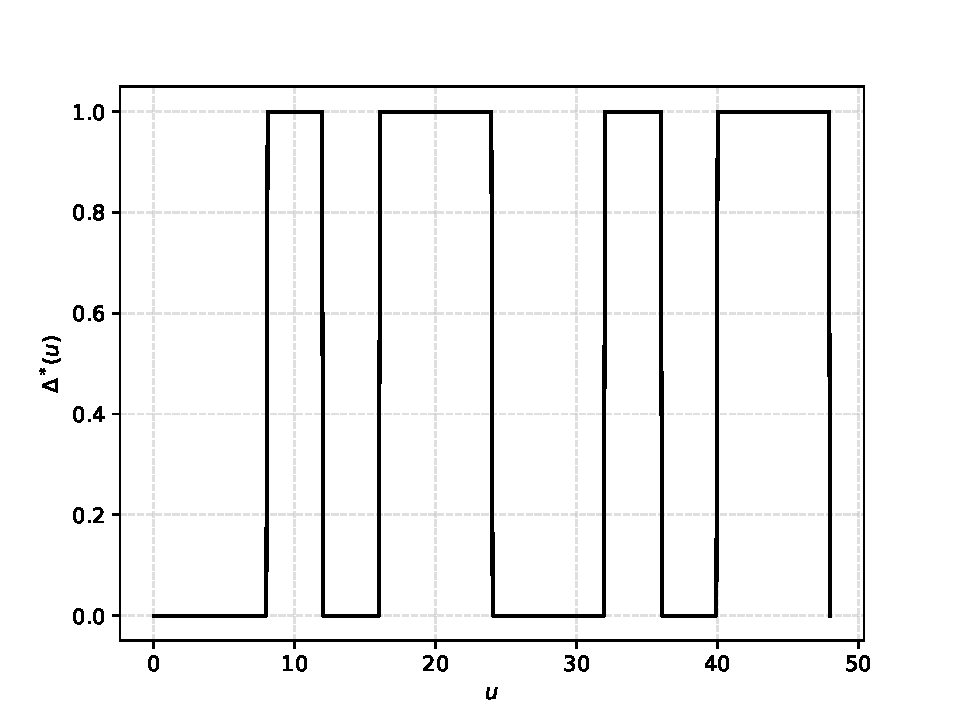
\includegraphics[width=\linewidth]{/home/tempdata/repos/thesis/static/misc/delta8m12q.pdf}
  \end{minipage}
  \hfill
  \begin{minipage}[t]{0.48\textwidth}
    \centering
    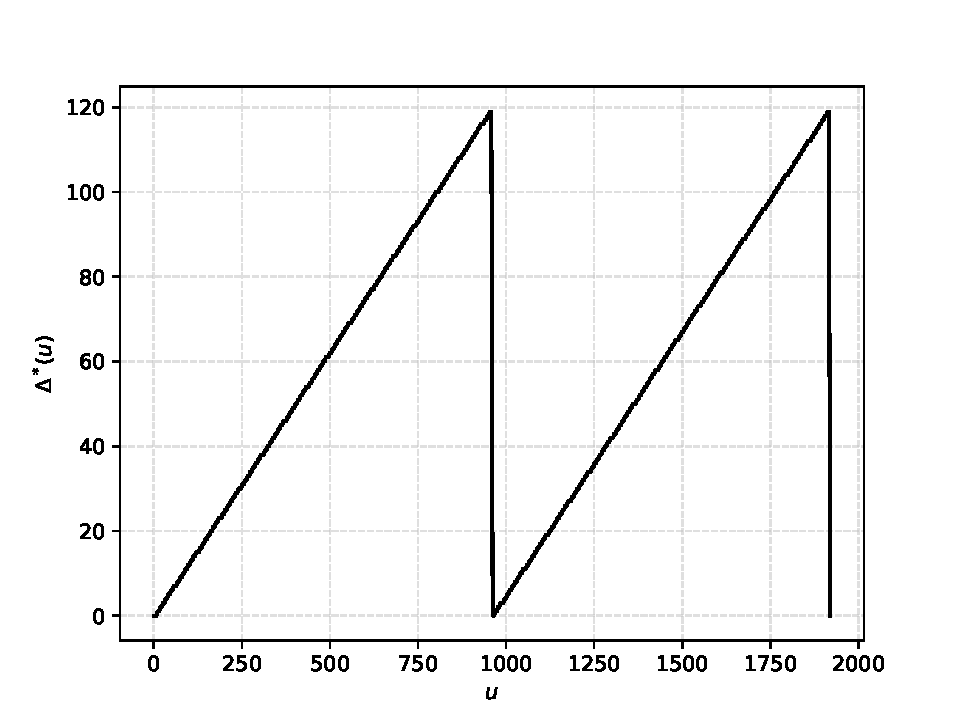
\includegraphics[width=\linewidth]{/home/tempdata/repos/thesis/static/misc/delta008m960q.pdf}
  \end{minipage}

  \caption{Número de capas a revisar en función del presupuesto. \textit{Izquierda: }Para los
	  parámetros $m = 8$ y $q^* = 12$ encontramos que hay un máximo de una capa a revisar.
	\textit{Derecha: } A medida que $m$ se vuelve fraccionario, las capas a revisar aumentan. En
		este caso tenemos $m = 0.08$ y $q^* = 960$.}
  \label{fig:m:ex}
\end{figure}

Observaremos en el análisis de resultados que el número de capas enteras que nuestro algoritmo
revisa en realidad disminuye a medida que aumenta el presupuesto $u$.

En esta segunda parte de la sección, demostraremos que para un presupuesto $u$ suficientemente
grande, la solución del problema \eqref{theory:formulation} se encuentra en la $\eta$-ésima capa
entera donde, como siempre, $\eta$ es recuperada del lema \ref{phase-1:lemma:eta}. Este resultado
será análogo al teorema \ref{infinite:th:complexity}. No obstante, para lograr aquello, necesitamos
de un par de definiciones y lemas preliminares.

Para motivar al lector, primero mostramos que existe una vecindad fija de todo punto en $\R^n$ de
manera que esa vecindad contiene al menos un punto entero. Esto es especificado en el teorema
\ref{lemma:ball-cover}.

Luego, observamos que el ``trozo'' no negativo de una capa entera $H_{\vec{q},
k\norm{\vec{q}}^{-2}}$ crece a medida que $k$ aumenta. Así pues, si $k$ es lo suficientemente
grande, habrá un punto sobre ese trozo no negativo cuya vecindad también se encuentra contenida en
ese trozo y, por lo tanto, habrá un punto entero no negativo sobre ese trozo. Esto es especificado
en el teorema \ref{th:intsimplex}.

Finalmente, relacionamos el punto entero que se encuentra sobre el pedazo no negativo de
$H_{\vec{q}, k\norm{\vec{q}}^{-2}}$ con el problema \eqref{theory:formulation}. Así pues, concluimos
esta sección con los teoremas \ref{th:intnonneg1} y \ref{th:intnonneg2}.

\begin{definition}
	\label{fin:def:ball}
	Sea $\vec{q} \in \Z^n$ un vector coprimo y sea $k$ un entero. Entonces definimos la
	\textbf{bola cerrada} sobre la $k$-ésima capa entera $H_{\vec{q}, k\norm{\vec{q}}^{-2}}$ con
	radio $r > 0$ y centro $\vec{x} \in H_{\vec{q}, k\norm{\vec{q}}^{-2}}$ como
	\begin{equation}
		\label{eq:k-ball}
		B_r^{(k)}(\vec{x}) \coloneq \lbrace \vec{y} \in \R^n \colon \norm{\vec{y} - \vec{x}} \leq r
		\rbrace \cap H_{\vec{q}, k \norm{\vec{q}}^{-2}}.
	\end{equation}
\end{definition}
% TODO: mostrar una imagen con una bola.
\begin{theorem}
	\label{lemma:ball-cover}
	Sea $\vec{q} \in \Z^n$ un vector coprimo y supongamos que $q_n \neq 0$. Sea $k$ un entero.
	Entonces existe $r > 0$ tal que la familia de bolas
	\begin{equation*}
		\left\lbrace B_r^{(k)}(\vec{x}) \colon \vec{x} \in H_{\vec{q}, k\norm{\vec{q}}^{-2}} \cap
			\Z^n \right\rbrace
	\end{equation*}
	es una cubierta de la $k$-ésima capa entera $H_{\vec{q}, k\norm{\vec{q}}^{-2}}$.
\end{theorem}
\begin{proof}
	Como $q_n \neq 0$, recordemos del teorema \eqref{th:lattice} que
	\begin{equation*}
		\vec{x} \in H_{\vec{q}, k\norm{\vec{q}}^{-2}} \cap \Z^n \iff \vec{x} = k\vec{\nu} + M\vec{t}
	\end{equation*}
	para algún vector $\vec{t} \in \Z^{n-1}$, donde recuperamos $\vec{\nu}$ y $M$ de
	\eqref{eq:vec-omega} y \eqref{eq:mat-T}, respectivamente. Así, tenemos
	\begin{equation*}
		\left\lbrace B_r^{(k)}(\vec{x}) \colon \vec{x} \in H_{\vec{q}, k\norm{\vec{q}}^{-2}} \cap
			\Z^n \right\rbrace
			=
		\left\lbrace B_r^{(k)}(k\vec{\nu} + M\vec{t}) \colon \vec{t} \in \Z^{n-1} \right\rbrace.
	\end{equation*}
	Por la definición \ref{fin:def:ball} sabemos que $B_r^{(k)}(k\vec{\nu} + M\vec{t}) \subseteq H_{\vec{q},
	k\norm{\vec{q}}^{-2}}$ para todo $r > 0$ y para todo $\vec{t} \in \Z^{n-1}$. Luego, para
	cualquier $r > 0$ tenemos
	\begin{equation}
		\label{eq:ball-cover:1}
		\bigcup_{\vec{t} \in \Z^{n-1}}B_r^{(k)}(k\vec{\nu} + M\vec{t}) \subseteq
		H_{\vec{q}, k\norm{\vec{q}}^{-2}}.
	\end{equation}
	Ahora bien, sea $\vec{y}$ un punto sobre la $k$-ésima capa entera. Por el lema \ref{lemma:iso2}
	sabemos que las columnas de $M$ son linealmente independientes, y entonces existe $\vec{t} \in
	\R^{n-1}$ tal que
	\begin{equation*}
		\vec{y} = k\vec{\nu} + M\vec{t}.
	\end{equation*}
	Sea $\lfloor \vec{t} \rceil \in \Z^{n-1}$ el vector resultante de redondear cada entrada de
	$\vec{t}$ al entero más cercano. Luego, $\vec{t} = \lfloor \vec{t} \rceil + \vec{\delta}$,
	para alguna $\vec{\delta} \in \R^{n-1}$ que satisface $\norm{\vec{\delta}}_{\infty} \leq 1/2$.
	Definamos
	\begin{equation*}
		\vec{x} \coloneq k\vec{\nu} + M\lfloor \vec{t} \rceil \in \Z^{n-1},
	\end{equation*}
	de donde se sigue que
	\begin{align}
		\norm{\vec{y} - \vec{x}}^{2} 
		&= \norm{M\vec{\delta}}^{2} \nonumber \\
		&\leq \sum_{i=1}^{n-1}|\delta_i|^2 \norm{M\vec{e}_i}^{2} \nonumber \\
		&\leq \frac{1}{4}\sum_{i=1}^{n-1} \norm{M\vec{e}_i}^{2} \label{eq:alt-M-bound} \\
		&= \frac{1}{4}\norm{M}_F^2, \nonumber
	\end{align}
	donde $\norm{M}_F$ denota la norma Frobenius de $M$. Por lo tanto, si definimos
	\begin{equation}
		\label{eq:radius}
		r \coloneq \frac{1}{2}\norm{M}_F,
	\end{equation}
	encontramos que $\vec{y} \in B_r^{(k)}(\vec{x})$. Luego, como $\vec{y} \in H_{\vec{q},
	k\norm{\vec{q}}^2}$ fue genérico, tenemos que si $r$ está definido por \eqref{eq:radius},
	entonces
	\begin{equation}
		\label{eq:ball-cover:2}
		H_{\vec{q}, k\norm{\vec{q}}^{-2}} \subseteq
		\bigcup_{\vec{t} \in \Z^{n-1}}B_r^{(k)}(k\vec{\nu} + M\vec{t}).
	\end{equation}
	Juntando esto con (\ref{eq:ball-cover:1}) obtenemos lo que queríamos demostrar.
\end{proof}

Lo que se encuentra a continuación se encarga de formalizar y caracterizar lo que nos referíamos
anteriormente como ``trozo no negativo'' de la $k$-ésima capa entera. Todas las definiciones fueron
tomadas de \cite{boyd} a excepción del baricentro, mientras que las demostraciones de los lemas y
teoremas fueron realizadas completamente por el autor.
\begin{definition}
	\label{def:aff}
	Sean $\vec{v}_1, \ldots, \vec{v}_m \in \R^n$ una colección de vectores,
	entonces definimos su \textbf{combinación afina} a partir de
	\begin{equation*}
		\aff\braces{\vec{v}_1, \ldots, \vec{v}_m} \coloneq \braces{\theta_1\vec{v}_1 + \cdots + \theta_k\vec{v}_k
		\colon \theta_1 + \cdots + \theta_m = 1}.
	\end{equation*}
\end{definition}

\begin{lemma}
	\label{lemma:aff}
	Sean $\vec{v}_1, \ldots, \vec{v}_m \in \R^n$ una colección de vectores. Entonces
	\begin{equation*}
		\aff\braces{\vec{v}_1, \ldots, \vec{v}_m} = \vec{v}_j + \gen\braces{\vec{v}_i -
		\vec{v}_j}_{i=1}^{n} = \vec{v}_j + \gen\braces{\vec{v}_i - \vec{v}_j}_{i\neq j}.
	\end{equation*}
\end{lemma}
\begin{proof}
	Puesto que $\vec{v}_j - \vec{v}_j = \vec{0}$, se sigue inmediatamente que
	\begin{equation*}
		\vec{v}_j + \gen\braces{\vec{v}_i - \vec{v}_j}_{i = 1}^{n}
		=
		\vec{v}_j + \gen\braces{\vec{v}_i - \vec{v}_j}_{i \neq j}.
	\end{equation*}
	Sean $\theta_1, \ldots, \theta_m$ escalares tales que $\theta_1 + \cdots + \theta_m = 1$. Por un
	lado, tenemos
	\begin{align*}
		\sum_{i=1}^{m}\theta_i\vec{v}_i
		&= \sum_{i=1}^{m}\theta_i\vec{v}_j + \sum_{i=1}^{m}\theta_i(\vec{v}_i - \vec{v}_j)  \\
		&= \vec{v}_j  + \sum_{i \neq j}\theta_i(\vec{v}_i - \vec{v}_j).
	\end{align*}
	De donde se sigue que $\aff\braces{\vec{v}_1, \ldots, \vec{v}_m} \subseteq \vec{v}_j +
	\gen\braces{\vec{v}_i - \vec{v}_j}_{i \neq j}$.

	Ahora bien, sea $\braces{\lambda_i}_{i \neq j}$ un conjunto de $m - 1$ escalares y definamos
	\begin{equation*}
		\lambda_j = 1 - \sum_{i \neq j}\lambda_i.
	\end{equation*}
	Observemos que $\lambda_1 + \cdots + \lambda_m = 1$ y, además,
	\begin{align*}
		\vec{v}_j + \sum_{i \neq j}\lambda_i(\vec{v}_i - \vec{v}_j)
		&= \left(1 - \sum_{i \neq j}\lambda_i\right)\vec{v}_j
		+ \sum_{i \neq j}\lambda_i\vec{v}_i \\
		&= \lambda_j\vec{v}_j + \sum_{i \neq j}\lambda_i\vec{v}_i \\
		&= \sum_{i = 1}^{m}\lambda_i\vec{v}_i.
	\end{align*}
	De donde se sigue que $\vec{v}_j + \gen\braces{\vec{v}_i - \vec{v}_j}_{i \neq j} \subseteq
	\aff\braces{\vec{v}_1, \ldots, \vec{v}_m}$. Puesto que hemos mostrado ambas contenciones,
	obtenemos lo que queríamos demostrar.
\end{proof}
\begin{example}
	\label{ex:aff}
	% Si $\vec{q}$ es un vector coprimo que satisface $q_n \neq 0$, entonces la $k$-ésima capa entera
	% $H_{\vec{q}, k\norm{\vec{q}}^{-2}}$ es la combinación afina de un conjunto de vectores. En
	% efecto, sabemos del teorema \ref{th:lattice} que el vector $\vec{\nu}$ (ver
	% \eqref{eq:vec-omega}) junto con las columnas $\vec{m}_1, \ldots, \vec{m}_{n-1}$ de M (ver
	% \eqref{eq:mat-T}) forman una base de la red $\Z^n$ y, por extensión, del espacio vectorial
	% $\R^n$.

	% De esta manera tenemos $\vec{x} \in H_{\vec{q}, k\norm{\vec{q}}^{-2}}$ si y solo si $\vec{x} =
	% k\vec{\nu} + M\vec{t}$ para alguna $\vec{t} \in \R^{n-1}$. Así pues,
	% \begin{equation*}
	% 	H_{\vec{q}, k\norm{\vec{q}}^{-2}} = k\vec{\nu} + \gen\braces{\vec{m}_i}
	% 	= k\vec{\nu} + \gen\braces{(\vec{m}_i + k\vec{\nu}) - k\vec{\nu}}.
	% \end{equation*}
	% Por el lema \ref{lemma:aff} sabemos entonces que la $k$-ésima capa entera es la combinación
	% afina de los vectores $k\vec{\nu}, \vec{m}_1 + k\vec{\nu}, \ldots, \vec{m}_{n-1} + k\vec{\nu}$.

	Si $\vec{q} > \vec{0}$ es un vector coprimo y $k$ un entero positivo, entonces la $k$-ésima capa
	entera $H_{\vec{q}, k\norm{\vec{q}}^{-2}}$ es la combinación afina de un conjunto de vectores.
	En efecto, recordemos de la definición \ref{phase-1:def:c-layer} que esta capa entera es
	simplemente un hiperplano afino. Como $\vec{q}$ es el vector normal a este hiperplano, se sigue
	que puede ser escrito como $\vec{v} + \ker{\vec{q} \mapsto \vec{q}^T\vec{x}}$ para alguna
	$\vec{v} \in H_{\vec{q}, k\norm{\vec{q}}^{-2}}$.

	Sean $\vec{u}_1, \ldots, \vec{u}_n$ las intersecciones de la $k$-ésima capa entera con cada uno
	de los ejes. Es decir, sean, para cada $i \in \braces{1, \ldots, n}$,
	\begin{equation}
		\label{def:u-basis}
		\vec{u}_i \coloneq \frac{k}{q_i}\vec{e}_i.
	\end{equation}
	Como cada $\vec{u}_i$ está en la $k$-ésima capa entera, se verifica que $\vec{q}^T\vec{u}_i = k$
	y por lo tanto $\vec{u}_i - \vec{u}_j \in \ker{\vec{q} \mapsto \vec{q}^T\vec{x}}$. No es difícil
	ver entonces que el conjunto de vectores $\braces{\vec{u}_i - \vec{u}_j}_{i \neq j}$ forma una
	base del espacio nulo de la transformación lineal $\vec{q} \mapsto \vec{q}^T\vec{x}$, por lo que
	obtenemos
	\begin{equation*}
		H_{\vec{q}, k\norm{\vec{q}}^{-2}} = \vec{u}_j + \gen\braces{\vec{u}_i - \vec{u}_j}_{i \neq
		j}.
	\end{equation*}
	Por el lema \ref{lemma:aff} concluimos que la $k$-ésima capa entera es la combinación
	afina de los vectores $\vec{u}_1, \ldots, \vec{u}_n$.
\end{example}

\begin{definition}
	\label{def:simplex}
	Sean $\vec{v}_1, \ldots, \vec{v}_m \in \R^n$ vectores linealmente independientes. Entonces
	definimos el \textbf{símplice} $\sigma$ como la combinación convexa de estos vectores:
	\begin{equation*}
		\sigma = \conv\braces{\vec{v}_1, \ldots, \vec{v}_m}
		\coloneq
		\braces{\theta_i\vec{v}_1 + \cdots + \theta_k\vec{v}_m
		\colon \theta_1 + \cdots + \theta_m = 1, \theta_i \geq 0}.
	\end{equation*}
	Decimos entonces que $\sigma$ es generado por $\vec{v}_1, \ldots, \vec{v}_n$. También definimos
	la \textbf{$j$-ésima faceta} $\sigma_j$ de $\sigma$ como el símplice generado por los vectores
	$\braces{\vec{v}_i}_{i \neq j}$.
\end{definition}
\begin{observation}
	Comparando con la definición \ref{def:aff}, encontramos que todo símplice $\sigma$ generado por
	$\vec{v}_1, \ldots, \vec{v}_m$ está contenido en la combinación afina de estos vectores. Es
	decir,
	\begin{equation}
		\label{aff:contention}
		\conv\braces{\vec{v}_1, \ldots, \vec{v}_m} \subseteq
		\aff\braces{\vec{v}_1, \ldots, \vec{v}_m}.
	\end{equation}
\end{observation}
\begin{observation}
	Si $\sigma$ es un símplice generado por $m$ vectores, entonces tiene $\binom{m}{m-1} = m$
	facetas. Tomaremos por hecho, puesto que de otra manera arriesgamos desviarnos por una tangente,
	que estas facetas constituyen la frontera relativa del símplice. Es decir, tomaremos por hecho
	que las facetas constituyen las ``aristas'' o ``caras'' de $\sigma$.
\end{observation}

\begin{lemma}
	\label{lemma:sigmachar1}
	Sea $\vec{q} > \vec{0}$ un vector coprimo y sea $H_{\vec{q}, k\norm{\vec{q}}^{-2}}$ la
	$k$-ésima capa entera, con parámetro $k$ positivo. Consideremos el símplice $\sigma$ generado por
	los vectores definidos en \eqref{def:u-basis}, entonces
	\begin{equation*}
		\sigma = H_{\vec{q}, k\norm{\vec{q}}^{-2}} \cap \R^n_{\geq \vec{0}}.
	\end{equation*}
\end{lemma}
\begin{proof}
	En el Ejemplo \ref{ex:aff} mostramos que
	\begin{equation*}
		\label{eq:aff-layer}
		H_{\vec{q}, k\norm{\vec{q}}^{-2}} = \aff\braces{\vec{u}_1, \ldots, \vec{u}_n}.
	\end{equation*}
	Sea $\vec{x} \in \sigma$, de la definición \ref{def:simplex} y de \eqref{aff:contention} encontramos
	que $\vec{x}$ se encuentra en la $k$-ésima capa entera. Además, existen escalares $\theta_1,
	\ldots, \theta_n$ no negativos tales que
	\begin{equation*}
		\vec{x} = \theta_1\vec{u}_1 + \cdots + \theta_n\vec{u}_n
		= k\begin{pmatrix}
			\theta_1 / q_1 \\
			\vdots \\
			\theta_n / q_n
		\end{pmatrix}.
	\end{equation*}
	Como $\vec{q} > \vec{0}$ y $k > 0$ por hipótesis, tenemos que $\vec{x} \geq \vec{0}$, lo que
	implica que $\vec{x} \in H_{\vec{q}, k\norm{\vec{q}}^{-2}} \cap \R^n_{\geq \vec{0}}$.

	El otro lado de la contención se muestra de manera completamente análoga.
\end{proof}

En el contexto del problema \eqref{theory:formulation}, sabemos que si $\sigma$ es generado por los
vectores en \eqref{def:u-basis} entonces, por el lema anterior, todo punto entero sobre $\sigma$ es
un punto factible siempre que $0 < k \leq \eta$, donde recuperamos $\eta$ del lema
\ref{phase-1:lemma:eta}. Nos gustaría entonces garantizar la existencia de tal punto entero.

Adoptamos la siguiente estrategia: nos concentramos en un punto $\vec{x} \in \sigma$ y abrimos una
bola (ver definición \ref{fin:def:ball}) con radio dado por \eqref{eq:radius}. Si esa bola está
contenida en el símplice $\sigma$, entonces el teorema \ref{lemma:ball-cover} garantiza la
existencia de un punto entero sobre $\sigma$. Por el lema anterior, garantizaríamos la
existencia de un punto entero no negativo sobre la $k$-ésima capa entera.

Lo que se encuentra a continuación es un análisis para determinar qué tan grande debe ser $k$ para
asegurar que la bola de radio \eqref{eq:radius} esté contenida en el símplice $\sigma$, dado que la
bola está centrada en un punto particular, a saber, en el baricentro del símplice.

\begin{definition}
	Sea $\sigma$ un símplice generado por $\vec{v}_1, \ldots, \vec{v}_m \in \R^n$, definimos su
	\textbf{baricentro} $\est{\sigma}$ como
	\begin{equation*}
		\est{\sigma} \coloneq \frac{1}{m} \sum_{i=1}^{m}\vec{v}_i.
	\end{equation*}
\end{definition}
\begin{observation}
	El baricentro $\est{\sigma}$ es un elemento de $\sigma$. Esto se debe a que $\est{\sigma}$ es la
	combinación convexa de $\vec{v}_1, \ldots, \vec{v}_m$, donde $\theta_1 = \cdots = \theta_m =
	\frac{1}{m}$.
\end{observation}

\begin{definition}
	\label{def:r-sigma}
	Sea $\sigma$ un símplice y sea $\est{\sigma}$ su baricentro. Entonces definimos el \textbf{radio
	de la bola inscrita} en $\sigma$ con centro $\est{\sigma}$ como
	\begin{equation}
		\label{eq:def:r-sigma}
		r_\sigma \coloneq \max \lbrace r > 0 \colon B_r^{(k)}(\est{\sigma})
		\subseteq \sigma \rbrace,
	\end{equation}
	donde $B_r^{(k)}(\est{\sigma})$ está dada en la definición \ref{fin:def:ball}.
\end{definition}

Encontraremos que el radio de la bola inscrita está dado por el mínimo de las distancias
entre el baricentro del símplice con cada una de sus facetas. Puesto que $\est{\sigma}_j \in
\sigma_j$, sabemos bien por álgebra lineal, bien por optimización, que la distancia entre $\sigma$ y
su $j$-ésima faceta $\sigma_j$ es
\begin{equation}
	\label{eq:dist:v1}
	d(\est{\sigma}, \sigma_j) = |\uvec{\mu}_j^T(\est{\sigma} - \est{\sigma}_j)|,
\end{equation}
donde $\uvec{\mu}_j$ es un vector unitario y normal a la $j$-ésima faceta.

\begin{lemma}
	\label{mu:orth}
	Sean $\vec{q} > \vec{0}$, $k > 0$ y retomemos el símplice $\sigma$ generado por los vectores
	$\braces{\vec{u}_i}_{i=1}^{n}$ en \eqref{def:u-basis}. Definamos, para cada $j \in \braces{1,
	\ldots, n}$,
	\begin{equation}
		\label{eq:normal}
		\vec{\mu}_j \coloneq \vec{u}_j - \frac{\vec{q}^T\vec{u}_j}{\vec{q}^T\vec{q}}\vec{q}
		= \vec{u}_j - \frac{k}{\norm{\vec{q}}^2}\vec{q}.
	\end{equation}
	Entonces $\vec{\mu}_j$ es un vector normal a la $j$-ésima faceta $\sigma_j$ del símplice
	$\sigma$.
\end{lemma}
\begin{proof}
	Debemos mostrar que si $\vec{x} \in \sigma_j$, entonces $\vec{\mu}_j^T\vec{y} = 0$ para todo
	$\vec{y} \in \sigma_j - \vec{x}$. Por la definición \ref{def:simplex}, tenemos que los vectores
	$\braces{\vec{u}_i}_{i \neq j}$ generan la $j$-ésima faceta $\sigma_j$, y entonces basta mostrar
	que $\vec{\mu}_j^T\vec{y} = 0$ para todo $\vec{y} \in \sigma_j - \vec{u}_m$ con $m \neq j$.

	Sea, pues, $m \in \braces{1, \ldots, n} \setminus \braces{j}$. Tenemos de las definiciones
	\ref{def:aff} y \ref{def:simplex}, así como del lema \ref{lemma:aff} que
	\begin{equation*}
		\sigma_j = \conv\braces{\vec{u}_i}_{i \neq j} \subseteq
		\aff\braces{\vec{u}_i}_{i \neq j}
		= \vec{u}_m + \gen\braces{\vec{u}_i - \vec{u}_m}_{i \neq j}.
	\end{equation*}
	De donde obtenemos
	\begin{equation*}
		\sigma_j - \vec{u}_m \subseteq \gen\braces{\vec{u}_i - \vec{u}_m}_{i \neq j},
	\end{equation*}
	así que basta mostrar que $\vec{\mu}_j^T(\vec{u}_i - \vec{u}_m) = 0$ para todo $i \neq j$ Cabe
	mencionar que los vectores $\braces{\vec{u}_i}_{i=1}^{n}$ son ortogonales entre sí (ver
	\eqref{def:u-basis}). Sustituyendo con la definición de $\vec{\mu}_j$ en la hipótesis, obtenemos
	\begin{align*}
		\vec{\mu}_j^T(\vec{u}_i - \vec{u}_m)
		&=
		\vec{u}_j^T\vec{u}_i - \vec{u}_j^T\vec{u}_m - \frac{k}{\norm{\vec{q}}^2}(\vec{q}^T\vec{u}_i
		- \vec{q}^T\vec{u}_m) \\
		&= 0 - 0 -\frac{k}{\norm{\vec{q}}^2}(k - k) \\
		&= 0.
	\end{align*}
	De esta manera, concluimos que $\vec{\mu}_j$ es un vector normal a $\sigma_j$.
\end{proof}

Ahora que encontramos vectores normales $\vec{\mu}_j$ para cada faceta $\sigma_j$, podemos
simplificar un poco más \eqref{eq:dist:v1}. Aprovechando el hecho de que
$\braces{\vec{u}_i}_{i=1}^{n}$ son todos ortogonales entre sí, obtenemos cálculos simples:
\begin{align*}
	\vec{\mu}_j^T\est{\sigma}
	&=
	\left(\vec{u}_j - \frac{k}{\norm{\vec{q}}^2}\vec{q}\right)^T \frac{1}{n}\sum_{i=1}^{n}\vec{u}_i \\
	&=
	\frac{1}{n}\sum_{i=1}^{n}\vec{u}_j^T\vec{u}_i - \frac{k}{n\norm{\vec{q}}^2}
	\sum_{i=1}^{n}\vec{q}^T\vec{u}_i \\
	&= \frac{1}{n}\norm{\vec{u}_j}^2 - \frac{k}{n\norm{\vec{q}}^2}\sum_{i=1}^{n}k \\
	&= \frac{k^2}{nq_j^2} - \frac{k^2}{\norm{\vec{q}}^2}.
\end{align*}
A través de un procedimiento similar, encontramos también que
\begin{equation}
	\label{eq:facetaux}
	\vec{\mu}_j^T\est{\sigma}_j = -\frac{k}{\norm{\vec{q}}^2},
\end{equation}
y por lo tanto
\begin{equation}
	\label{eq:signed}
	\vec{\mu}_j^T(\est{\sigma} - \est{\sigma}_j) = \frac{k^2}{nq_j^2}.
\end{equation}
Más adelante normalicaremos $\vec{\mu}$ de manera que este vector sea unitario. Cabe resaltar el
hecho de que el lado derecho \eqref{eq:signed} es positivo. Geométricamente, lo anterior implica
que los vectores normales $\vec{\mu}_j$ de cada faceta $\sigma_j$ apuntan hacia el interior relativo
del símplice $\sigma$. Esto sugiere una caracterización alternativa de $\sigma$ que nos permite
interpretarlo como un poliedro.
\begin{lemma}
	\label{lemma:sigmachar2}
	Sea $\vec{q} > \vec{0}$ un vector coprimo y sea $\sigma$ el símplice generado por los vectores
	definidos en \eqref{def:u-basis}, con $k > 0$. Entonces
	\begin{equation}
		\label{eq:sigmachar2}
		\sigma = \bigcap_{j=1}^{n}
		\braces{\vec{x} \in \R^n \colon \uvec{\mu}_j^T(\vec{x} - \est{\sigma}_j) \geq 0}
		\cap H_{\vec{q}, k\norm{\vec{q}}^{-2}},
	\end{equation}
	donde $\uvec{\mu}_j$ es el vector $\vec{\mu}_j$ definido en \eqref{eq:normal} normalizado.
\end{lemma}
\begin{proof}
	Denotemos por $\braces{\vec{u}_i}_{i=1}^{n}$ los vectores ortogonales definidos en
	\eqref{def:u-basis}. Como $\uvec{\mu}_j$ es el vector $\vec{\mu}_j$ normalizado, se sigue que
	\begin{equation*}
		\braces{ \vec{x} \in \R^n \colon \uvec{\mu}_j^T(\vec{x} - \est{\sigma}_j) \geq 0}
		=
		\braces{ \vec{x} \in \R^n \colon \vec{\mu}_j^T(\vec{x} - \est{\sigma}_j) \geq 0},
	\end{equation*}
	y entonces podemos trabajar con $\vec{\mu}_j$ sin normalizarlo. 

	Sea $\vec{x} \in \sigma$. Por el lema \ref{lemma:sigmachar1} sabemos que
	$\vec{x}$ se encuentra en la $k$-ésima capa entera. También sabemos que existen escalares no
	negativos $\theta_1, \ldots, \theta_n$ que suman 1 y que satisfacen $\vec{x} = \theta_1\vec{u}_1
	+ \cdots + \theta_n\vec{u}_n$. Tenemos entonces
	\begin{align*}
		\vec{\mu}_j^T\vec{x}
		&=
		\left(\vec{u}_j - \frac{k}{\norm{\vec{q}}^2}\vec{q}\right)^T
		\left(\theta_j\vec{u}_j + \sum_{i \neq j}\theta_i\vec{u}_i\right) \\
		&= \theta_j\norm{\vec{u}_j}^2 - \frac{k}{\norm{\vec{q}}^2}\sum_{i \neq j}
		\theta_i\vec{q}^T\vec{u}_i \\
		&= \theta_j\frac{k^2}{q_j^2} - \frac{k}{\norm{\vec{q}}^2}\sum_{i \neq j}k\theta_i \\
		&= \theta_j\frac{k^2}{q_j^2} - \frac{k^2}{\norm{\vec{q}}^2}(1 - \theta_j) \\
		&= \theta_j\left(\frac{k^2}{q_j^2} + \frac{k^2}{\norm{\vec{q}}^2}\right)
		- \frac{k^2}{\norm{\vec{q}}^2}.
	\end{align*}
	Retomamos de \eqref{eq:facetaux} el valor de $\vec{\mu}_j^T\est{\sigma}_j$, así que obtenemos
	\begin{equation*}
		\vec{\mu}_j^T(\vec{x} - \est{\sigma}_j)
		= 
		\vec{\mu}_j^T\vec{x} - \vec{\mu}_j^T\est{\sigma}_j
		=
		\theta_j\left(\frac{k^2}{q_j^2} + \frac{k^2}{\norm{\vec{q}}^2}\right),
	\end{equation*}
	lo cual es no negativo para todo $j \in \braces{1, \ldots, n}$.

	Mostramos la otra contención por contrapositiva, así que supongamos que $\vec{x} \not\in
	\sigma$. Por el lema \ref{lemma:sigmachar1} se sigue o bien que $\vec{x} \not\in H_{\vec{q},
	k\norm{\vec{q}}^{-2}}$ o bien que $\vec{x} \not\in \R^n_{\geq \vec{0}}$. En el primer caso
	obtenemos inmediatamente que $\vec{x}$ no se encuentra en el lado derecho de
	\eqref{eq:sigmachar2}.

	Supongamos, pues, que $\vec{x}$ está en la $k$-ésima capa entera pero que tiene al menos una
	entrada negativa con respecto a la base canónica. Como $\braces{\vec{u}_i}_{i=1}^{n}$ es base de
	$\R^n$, existen escalares $\braces{\lambda_i}_{i=1}^{n}$ tales que
	\begin{equation*}
		\vec{x} = \sum_{i=1}^{n}\lambda_i\vec{u}_i.
	\end{equation*}
	Como las entradas de $\vec{u}_1, \ldots, \vec{u}_n$ son todas no negativas y $x_j < 0$ para
	alguna $j \in \braces{1, \ldots, n}$, se sigue que $\lambda_j < 0$. Observemos que
	\begin{align*}
		\vec{\mu}_j^T\vec{x}
		&=
		\sum_{i=1}^{n}\lambda_i\vec{\mu}_j^T\vec{u}_i \\
		&=
		\sum_{i=1}^{n}\lambda_i\left(\vec{u}_j - \frac{k}{\norm{\vec{q}}^2}\vec{q}\right)^T\vec{u}_i \\
		&=
		\sum_{i=1}^{n}\lambda_i\left(\vec{u}_j^T\vec{u}_i -
			\frac{k}{\norm{\vec{q}}^2}\vec{q}^T\vec{u}_i\right) \\
		&=
		\lambda_j\norm{\vec{u}_j}^2 - \frac{k^2}{\norm{\vec{q}}} \sum_{i=1}^{n}\lambda_i.
	\end{align*}
	Pero $\vec{x} \in H_{\vec{q}, k\norm{\vec{q}}^{-2}} = \aff\braces{\vec{u}_1, \ldots, \vec{u}_n}$
	(ver Ejemplo \ref{ex:aff}) y entonces los escalares $\lambda_1, \ldots, \lambda_n$ suman a 1.
	Sustituyendo,
	\begin{equation*}
		\vec{\mu}_j^T\vec{x} = \lambda_j\frac{k^2}{q_j^2} - \frac{k^2}{\norm{\vec{q}}^2},
	\end{equation*}
	retomando el valor de $\vec{\mu}_j^T\est{\sigma}_j$ en \eqref{eq:facetaux}, encontramos que
	\begin{equation*}
		\vec{\mu}_j^T(\vec{x} - \est{\sigma}_j) = \lambda_j\frac{k^2}{q_j^2} < 0
	\end{equation*}
	y entonces $\vec{x}$ no es elemento del semi-espacio $\braces{\vec{x} \colon
	\vec{\mu}_j^T(\vec{x} - \est{\sigma}_j) \geq 0}$, por lo que tampoco es elemento del lado
	derecho de \eqref{eq:sigmachar2}.
\end{proof}

\begin{theorem}
	\label{lemma:sigma-radius}
	Sea $\vec{q} > \vec{0}$ un vector coprimo y sea $\sigma$ el símplice generado por los vectores
	$\braces{\vec{u}_i}_{i=1}^{n}$ definidos en \eqref{def:u-basis}. Entonces el radio $r_\sigma$ de
	la bola inscrita (ver definición \ref{def:r-sigma}) en $\sigma$ con centro
	$\est{\sigma}$ está dado por
	\begin{equation*}
		r_\sigma = \min_{1 \leq j \leq n} d(\est{\sigma}, \sigma_j)
		= \min_{1 \leq j \leq n} \uvec{\mu}_j^T(\est{\sigma} - \est{\sigma}_j),
	\end{equation*}
	donde $\uvec{\mu}_j$ es el vector $\vec{\mu}_j$ definido en \eqref{eq:normal} normalizado.
\end{theorem}
\begin{proof}
	Como $\est{\sigma} \in \sigma$, tenemos del lema \ref{lemma:sigmachar2} que
	$\vec{\mu}_j^T(\est{\sigma} - \est{\sigma}_j) \geq 0$ y, por lo tanto, deducimos de \eqref{eq:dist:v1}
	que la distancia entre $\est{\sigma}$ y la $j$-ésima faceta $\sigma_j$ es
	\begin{equation}
		\label{eq:dist}
		d(\est{\sigma}, \sigma_j) = \uvec{\mu}_j^T(\est{\sigma} - \est{\sigma}_j).
	\end{equation}

	Supongamos que $r \leq d(\est{\sigma}, \sigma_j)$ para todo $j \in \braces{1, \ldots, n}$ y sea
	$\vec{x} \in B_r^{(k)}(\est{\sigma})$. Observemos que
	\begin{align*}
		\uvec{\mu}_j^T(\vec{x} - \est{\sigma}_j)
		&= 
		\uvec{\mu}_j^T(\vec{x} - \est{\sigma})
		+
		\uvec{\mu}_j^T(\est{\sigma} - \est{\sigma}_j) \\
		&=
		\uvec{\mu}_j^T(\vec{x} - \est{\sigma}) + d(\est{\sigma}, \sigma_j).
	\end{align*}
	Por la desigualdad de Cauchy-Schwartz, tenemos
	\begin{equation*}
		\uvec{\mu}_j^T(\vec{x} - \est{\sigma}) \geq -\norm{\uvec{\mu}_j}\norm{\vec{x} -
		\est{\sigma}} \geq -r,
	\end{equation*}
	pues $\uvec{\mu}$ es unitario y $\vec{x} \in B_r^{(k)}(\est{\sigma})$. Así pues, tenemos
	\begin{equation*}
		\uvec{\mu}_j^T(\vec{x} - \est{\sigma}_j) \geq -r + d(\est{\sigma}, \sigma_j) \geq 0,
	\end{equation*}
	pues supusimos que $r \leq d(\est{\sigma}, \sigma_j)$ para todo $j \in \braces{1, \ldots, n}$.
	Además, como $\vec{x} \in B_r^{(k)}(\est{\sigma})$, por la definición \ref{fin:def:ball} tenemos
	que $\vec{x}$ se encuentra en la $k$-ésima capa entera. Así pues,
	\begin{equation*}
		\vec{x} \in
		\bigcap_{j=1}^{n}
		\braces{\vec{x} \in \R^n \colon \uvec{\mu}_j^T(\vec{x} - \est{\sigma}_j) \geq 0}
		\cap H_{\vec{q}, k\norm{\vec{q}}^{-2}} = \sigma,
	\end{equation*}
	donde la última igualdad se sigue del lema \ref{lemma:sigmachar2}. Así pues,
	$B_r^{(k)}(\est{\sigma}) \subseteq \sigma$ si $r \leq d(\est{\sigma}, \sigma_j)$ para toda $j
	\in \braces{1, \ldots, n}$. De la definición \ref{def:r-sigma} encontramos entonces que el radio
	$r_\sigma$ de la bola inscrita satisface
	\begin{equation}
		\label{r-sigma:down}
		r_\sigma \geq \min_{1 \leq j \leq n}d(\est{\sigma}, \sigma_j).
	\end{equation}

	Ahora bien, supongamos que $r > d(\est{\sigma}, \sigma_j)$ para alguna $j \in \lbrace 1, \ldots,
	n \rbrace$. Consideremos el punto $\vec{x} \in \sigma_j$ que satisface $d(\est{\sigma}, \sigma_j) =
	d(\est{\sigma}, \vec{x})$. Tal punto existe porque $\sigma_j$ es cerrado. Luego,
	$\norm{\vec{x} - \est{\sigma}} < r$. Entonces existe $\varepsilon > 0$ tal que
	\begin{equation*}
		\norm{(\vec{x} - \varepsilon\est{\mu}_j) - \est{\sigma}} \leq r,
	\end{equation*}
	lo que implica que $\vec{x} - \varepsilon\est{\mu}_j \in
	B_r^{(k)}(\est{\sigma})$. Observemos que
	\begin{equation*}
		\uvec{\mu}_j^T((\vec{x} - \varepsilon\uvec{\mu}_j) - \est{\sigma}_j)
		=
		\uvec{\mu}_j^T(\vec{x} - \est{\sigma}_j) - \varepsilon.
	\end{equation*}
	Pero $\vec{x}, \est{\sigma}_j \in \sigma_j$, así que $\vec{x} - \est{\sigma}_j \in \sigma_j -
	\est{\sigma}_j$. Del lema \ref{mu:orth} encontramos que
	\begin{equation*}
		\uvec{\mu}_j^T(\vec{x} - \est{\sigma}_j) = 0,
	\end{equation*}
	de donde obtenemos
	\begin{equation*}
		\uvec{\mu}_j^T((\vec{x} - \varepsilon\uvec{\mu}_i) - \est{\sigma}_j)
		= -\varepsilon < 0,
	\end{equation*}
	lo cual implica que $\vec{x} - \varepsilon\uvec{\mu}_j$ no se encuentra en el semi-espacio
	definido por $\braces{\vec{x} \colon \uvec{\mu}^T(\vec{x} - \est{\sigma}_j) \geq 0}$. Así pues,
	por el lema \ref{lemma:sigmachar2}, encontramos que $\vec{x} - \varepsilon\uvec{\mu}_j \not\in
	\sigma$. Pero $\vec{x} - \varepsilon\uvec{\mu}_j \in B_r^{(k)}(\est{\sigma})$. De aquí se desprende
	que $B_r^{(k)}(\est{\sigma}) \not\subseteq \sigma$ si $r > d(\est{\sigma}, \sigma_j)$ para
	alguna $j \in \braces{1, \ldots, n}$. De la definición \ref{def:r-sigma} obtenemos entonces
	\begin{equation}
		\label{r-sigma:up}
		r_\sigma \leq \min_{1 \leq j \leq n}d(\est{\sigma}, \sigma_j).
	\end{equation}

	De \eqref{r-sigma:down} y de \eqref{r-sigma:up} concluimos entonces con lo que queríamos
	demostrar.
\end{proof}

De \eqref{eq:dist:v1} tenemos
\begin{equation}
	\label{dist:v2}
	d(\est{\sigma}, \sigma_j) = \uvec{\mu}_j^T(\est{\sigma} - \est{\sigma}_j)
	= \frac{\vec{\mu}_j^T(\est{\sigma} - \est{\sigma}_j)}{\norm{\vec{\mu}_j}}.
\end{equation}
Recordemos de \eqref{eq:signed} que ya contamos con el numerador, así que ahora debemos calcular la
norma de $\vec{\mu}_j$. Tenemos
\begin{align*}
	\norm{\vec{\mu}_j}^2
	&= \vec{\mu}_j^T\vec{\mu}_j \\
	&=
	\left(\vec{u}_j - \frac{k}{\norm{\vec{q}}^2}\vec{q}\right)^T
	\left(\vec{u}_j - \frac{k}{\norm{\vec{q}}^2}\vec{q}\right) \\
	&=
	\norm{\vec{u}_j}^2 - 2\frac{k}{\norm{\vec{q}}^2}\vec{q}^T\vec{u}_j +
	\frac{k^2}{\norm{\vec{q}}^4}\vec{q}^T\vec{q} \\
	&= \frac{k^2}{q_j^2} - 2\frac{k^2}{\norm{\vec{q}}^2} + \frac{k^2}{\norm{\vec{q}}^2} \\
	&= \frac{k^2}{q_j^2} - \frac{k^2}{\norm{\vec{q}}^2}.
\end{align*}
De donde obtenemos
\begin{equation}
	\label{eq:den}
	\norm{\vec{\mu}_j} = k\sqrt{\frac{1}{q_j^2} - \frac{1}{\norm{\vec{q}}^2}}.
\end{equation}

Usando \eqref{eq:signed} y \eqref{eq:den} para sustituir en \eqref{dist:v2}, obtenemos
\begin{equation*}
	d(\est{\sigma}, \sigma_j) = \frac{k}{n} \cdot
	\frac{1}{q_j^2\sqrt{q_j^{-2} - \norm{\vec{q}}^{-2}}}
	= \frac{k}{n} \cdot \frac{1}{Q_j},
\end{equation*}
donde definimos $Q_j$ pertinentemente. Finalmente, del teorema \ref{lemma:sigma-radius} encontramos que
el radio $r_\sigma$ de la bola inscrita en el símplice $\sigma$ con centro
$\est{\sigma}$ está dado por
\begin{equation}
	\label{eq:sigma-radius}
	r_\sigma = \min_{1 \leq j \leq n} \braces{d(\est{\sigma}, \sigma_j)} = \frac{k}{n} \cdot
	\frac{1}{\max_{1 \leq j \leq n} \lbrace Q_j \rbrace}
\end{equation}

\begin{theorem}
	\label{th:intsimplex}
	Sea $\vec{q} > \vec{0}$ un vector coprimo y sea $k$ un entero positivo suficientemente grande.
	Entonces existe un punto entero sobre el símplice $\sigma$ generado por los vectores en
	\eqref{def:u-basis}.
\end{theorem}
\begin{proof}
	Sea $r$ el radio definido en \eqref{eq:radius} y sea $r_\sigma$ el radio definido en
	\eqref{eq:sigma-radius}. Por el teorema \ref{lemma:ball-cover} sabemos que existe un punto
	entero $\vec{x}$ en $B_r^{(k)}(\est{\sigma})$, y por el teorema \ref{lemma:sigma-radius} sabemos
	que la bola $B_{r_\sigma}^{(k)}(\est{\sigma})$ está contenida en $\sigma$. Entonces basta
	mostrar que existe $k$ suficientemente grande tal que $r \leq r_\sigma$, pues esto implicaría la
	contención de en medio en la cadena
	\begin{equation*}
		\vec{x} \in B_r^{(k)}(\est{\sigma}) \subseteq B_{r_\sigma}^{(k)}(\est{\sigma}) \subseteq \sigma.
	\end{equation*}
	De \eqref{eq:radius} y de \eqref{eq:sigma-radius} obtenemos que $r \leq r_\sigma$ si y solo si
	\begin{equation}
		\label{eq:eta-limit}
		k \geq \frac{n}{2}\norm{M}_F\max_{1 \leq j \leq n} \lbrace Q_j \rbrace,
	\end{equation}
	que es lo que queríamos demostrar.
\end{proof}
De \eqref{eq:eta-limit} parece que podemos concluir que hay una dependencia lineal entre la
dimensión $n$ y el parámetro de la capa entera $k$. No obstante, la norma $\norm{M}_F$ depende
implícitamente de $n$. Para ser más explícitos con respecto a esta dependencia, podemos rescatar de
\eqref{eq:alt-M-bound} la siguiente cota:
\begin{equation*}
	\frac{1}{4}\sum_{j=1}^{n-1}\norm{M\vec{e}_j}^2
	\leq
	\frac{n-1}{4}\max_{1 \leq j \leq n} \lbrace \norm{M\vec{e}_j}^2 \rbrace,
\end{equation*}
de donde reemplazaríamos la cota \eqref{eq:eta-limit} en el teorema \ref{th:intsimplex} por
\begin{equation*}
	k \geq \frac{n\sqrt{n-1}}{2} \max_{1 \leq j \leq n} \lbrace \norm{M\vec{e}_j} \rbrace \cdot
	\max_{1 \leq j \leq n} \lbrace Q_j \rbrace.
\end{equation*}
Esta cota, no obstante, es más grande que la propuesta inicialmente.

Además, el resultado que obtuvimos es más fuerte de lo que aparenta. Hemos encontrado una
cota inferior de manera que podamos asegurar la existencia de puntos enteros en una vecindad del
baricentro $\est{\sigma}$. Este punto no es especial, pues en realidad podemos realizar el mismo
procedimiento enfocándonos en otros puntos del símplice $\sigma$ para asegurar soluciones en sus
respectivas vecindades. Entonces, dependiendo del punto, podemos obtener mejores o peores cotas para
$k$. El punto más interesante es aquel que provee la cota inferior más pequeña\footnote{
	Una hipótesis del autor es que el baricentro $\est{\sigma}$ provee, en efecto, la mejor cota.
}.

De manera inmediata obtenemos también los siguientes teoremas. Cabe mencionar que estos resultados
solamente muestran la existencia de una solución entera $\vec{x}$ no negativa para la ecuación lineal
diofantina $\vec{q}^T\vec{x} = k$. Será en la Sección \ref{subsec:complex} que discutiremos cómo
encontrar esta solución.
\begin{theorem}
	\label{th:intnonneg1}
	Sea $\vec{q} > \vec{0}$ un vector coprimo. Entonces la ecuación lineal diofantina
	$\vec{q}^T\vec{x} = k$ tiene soluciones enteras no negativas para $k$ suficientemente grande.
\end{theorem}
\begin{proof}
	Consideremos el símplice $\sigma$ generado por los vectores en \eqref{def:u-basis} y supongamos
	que $k$ satisface la cota en \eqref{eq:eta-limit}.
	Por el teorema \ref{th:intsimplex} existe un punto entero no negativo $\vec{x} \in \sigma$, y
	esto implica que $x \in H_{\vec{q}, k\norm{\vec{q}}^{-2}}$ por el lema \ref{lemma:sigmachar1}.
	Luego, por el lema \ref{theory:lemma:utility}, $\vec{x}$ satisface la ecuación lineal diofantina
	$\vec{q}^T\vec{x} = k$.
\end{proof}
\begin{theorem}
	\label{th:intnonneg2}
	Sea $\vec{p} \in \R^n$ un vector esencialmente entero y supongamos que su múltiplo coprimo
	$\vec{q}$ tiene entradas estrictamente positivas. Entonces el problema
	\eqref{theory:formulation} se puede resolver a través de encontrar la solución de una sola
	ecuación lineal en $n$ incógnitas para un presupuesto $u$ suficientemente grande.
\end{theorem}
\begin{proof}
	Por la definición \ref{theory:def:rational} sabemos que existe un escalar $m$ tal que
	$\vec{p} = m\vec{q}$. Supongamos, sin pérdida de generalidad, que $m$ es positivo. Del lema
	\ref{phase-1:lemma:eta} tenemos que el entero $\eta$ parametriza la primera capa entera en
	satisfacer el presupuesto y que $\eta = \floor{u/m}$. Por el teorema \ref{th:intnonneg1} sabemos
	que si $\eta$ es suficientemente grande, entonces la ecuación lineal diofantina
	$\vec{q}^T\vec{x} = \eta$ tiene al menos una solución entera no negativa $\vec{x}$. Luego,
	$\vec{x}$ es factible para el problema \eqref{theory:formulation}, pero por la maximalidad de
	$\eta$ encontramos que $\vec{x}$ también es un punto óptimo. En conclusión, solo deviene
	necesario resolver una ecuación lineal diofantina para determinar la solución del problema
	\eqref{theory:formulation}.
\end{proof}

El teorema \ref{th:intnonneg1} junto con la cota \eqref{eq:eta-limit} provee, hasta donde llega el
conocimiento del autor, nuevas cotas superiores para los números de Frobenius\footnote{
	Véase el Problema de la Moneda en \url{https://en.wikipedia.org/wiki/Coin_problem}.
}. De manera resumida,
dada una colección de enteros $a_1, \ldots, a_n$ coprimos, el número de Frobenius es el entero $F$
más grande tal que $F$ no pueda ser expresado como una combinación lineal entera no negativa de
$a_1, \ldots, a_n$. Un estudio sobre cómo se compara esta colección de cotas con respecto a la
literatura existente, si bien interesante, queda fuera del propósito de esta tesis.

En último lugar, mencionamos que eventualmente es suficiente con revisar la primera capa entera. No
hemos demostrado, empero, que el número de capas enteras a revisar eventualmente decrece en cuanto
el presupuesto $u$ aumenta. Observaremos en el análisis de resultados que hay un patrón periódico y
decreciente en cuanto al número de capas enteras revisadas. Demostrar, en cambio, que este
comportamiento siempre se cumple es mucho más difícil y queda fuera del propósito de esta tesis.

\section{Construcción de soluciones}
\label{subsec:complex}

\noindent
Sea $\vec{p} \in \R^n$ un vector esencialmente entero y supongamos que las entradas de su múltiplo
coprimo $\vec{q}$ son todas estrictamente positivas. Supongamos, sin pérdida de generalidad, que el
escalar $m$ que satisface $\vec{p} = m\vec{q}$ es también positivo. Bastante hemos discutido sobre
cómo la solución del problema \eqref{theory:formulation} se traduce a la búsqueda de una solución
entera no negativa de la ecuación lineal diofantina $\vec{q}^T\vec{x} = k$ para alguna $k \leq \eta$,
donde $\eta$ es tomada del lema \ref{phase-1:lemma:eta}.

En esta sección presentamos los algoritmos \ref{algo:fin:helper} y \ref{algo:fin:dioph}, los cuales
se encargan de obtener estas soluciones enteras no negativas que tanto buscamos. Consecuentemente,
estos algoritmos se encargan de resolver el problema \eqref{theory:formulation}.

% En la segunda parte de esta sección discutimos de manera un tanto informal la complejidad
% algorítmica del Algoritmo \ref{algo:fin:dioph}. Por lo tanto, también discutimos, así como lo
% hicimos en el capítulo \ref{chap:inf}, sobre la complejidad del problema \eqref{theory:formulation}
% en el caso especial de que $\vec{q} > \vec{0}$.

\begin{theorem}
	\label{th:fin:helper:correct}
	El algoritmo \ref{algo:fin:helper} es correcto.
\end{theorem}
\begin{proof}
	Hacemos la demostración por inducción en la dimensión $n$ del vector $\vec{q}$. Supongamos, para
	el caso base, que $n = 2$. Luego, queremos encontrar soluciones enteras no negativas de la
	ecuación
	\begin{equation}
		\label{lemma:correct:base-case}
		q_1x_1 + q_2x_2 = k.
	\end{equation}
	Por hipótesis sabemos que $q_1$ y $q_2$ son coprimos. Luego, del teorema
	\ref{prerreq:th:construction} encontramos que las soluciones enteras de esta ecuación están
	dadas por
	\begin{equation}
		\label{lemma:correct:base-case:sol}
		\begin{cases}
			x_1 = kx_1' + q_2t, \\
			x_2 = kx_2' - q_1t, \\
		\end{cases}
	\end{equation}
	donde $t \in \Z$ es una variable libre, y $x_1', x_2'$ son los coeficientes de Bézout (c.f.
	definición \ref{prerreq:def:bezout}) de $q_1$ y $q_2$, respectivamente. Por claridad, escribimos
	$x_1'$ y $x_2'$ como $x_{n-1}'$ y $x_{n}'$ en la línea \ref{alg:fin:bez}. Despejando de estas
	soluciones, encontramos que existen soluciones no negativas si y solo si existe $t \in \Z$ que
	satisfaga
	\begin{equation*}
		\ceil{-\frac{kx_1'}{q_2}} \leq t \leq \floor{\frac{kx_2'}{q_1}}.
	\end{equation*}
	Los enteros $b_1$ y $b_2$ en las líneas \ref{alg:fin:b1} y \ref{alg:fin:b2} representan el
	lado izquierdo y derecho de estas desigualdades, respectivamente. De esta manera, el algoritmo
	devuelve \NIL~ si solo si este intervalo no está bien definido, es decir, si y solo si no existen
	soluciones enteras no negativas. Supongamos, pues, que este intervalo sí está bien definido.
	Entonces, podemos escoger que la variable libre $t$ sea $b_1$. Sustituyendo en
	\eqref{lemma:correct:base-case:sol} obtenemos una solución entera no negativa de la ecuación
	\eqref{lemma:correct:base-case} (líneas \ref{alg:fin:xprev} y \ref{alg:fin:xlast}) y entonces
	el algoritmo es correcto para $n = 2$.

	Haciendo uso de la hipótesis inductiva, queremos mostrar que el algoritmo también es correcto
	para $n \geq 3$ si lo es para $n - 1 \geq 2$. Entonces deseamos encontrar soluciones enteras no
	negativas de la ecuación \eqref{eq:dioph} Haciendo la misma sustitución que en
	\eqref{eq:dioph:first-step}, recordando que $q_1, \ldots, q_n$ son coprimos por hipótesis, que
	definimos $\omega_1 \coloneq k$, y renombrando las variables ($x$ en vez de $x_1$, $g$ en vez de
	$g_2$ y $\omega$ en vez de $\omega_2$), obtenemos la ecuación
	\begin{equation}
		\label{lemma:correct:eq}
		q_1x + g\omega = k.
	\end{equation}
	Observemos que, como $g_1 = 1$, el entero $g = \gcd{q_2/g_1, \ldots, q_n/g_1}$, es equivalente a
	lo que se encuentra en la línea \ref{alg:fin:g}. Por definición de $g$, tenemos que $q_1$ y $g$
	son coprimos (ver el lema \ref{prerreq:lemma:gcd}), así que por el teorema
	\ref{prerreq:th:construction} tenemos que las soluciones enteras de esta ecuación están dadas por
	\begin{equation}
		\label{lemma:correct:sol}
		\begin{cases}
			x = kx' + gt, \\
			\omega = k\omega' - q_1t,
		\end{cases}
	\end{equation}
	donde $t \in \Z$ es una variable libre, y $x', \omega'$ son los coeficientes de Bézout de $x,
	\omega$. Recordemos de \eqref{eq:dioph:first-step} que
	\begin{equation}
		\label{lemma:correct:eq-omega}
		\omega = \frac{q_2}{g}x_2 + \ldots + \frac{q_n}{g}x_n.
	\end{equation}
	Como $\vec{q} > \vec{0}$ por hipótesis, $g > 0$ porque el máximo común divisor siempre es
	positivo, y exigimos que $x_2, \ldots, x_n$ sean no negativos, debe ser el caso que $\omega$
	también sea no negativo. Luego, despejando de \ref{lemma:correct:sol}, existen soluciones no
	negativas de la ecuación \eqref{lemma:correct:eq} si y solo si existe $t \in \Z$ que satisfaga
	\begin{equation}
		\label{feas}
		\ceil{-\frac{kx'}{g}} \leq t \leq \floor{\frac{k\omega'}{q_1}}.
	\end{equation}
	Los enteros $b_1$ y $b_2$ en las líneas \ref{alg:fin:b11} y \ref{alg:fin:b21} representan el
	lado izquierdo y derecho de estas desigualdades, respectivamente. Si no existe tal variable
	libre $t \in \Z$ es porque el intervalo $[b_1, b_2]$ no está bien definido y por lo tanto $b_2 <
	b_1$. El algoritmo entonces salta a la línea \ref{alg:fin:return} y devuelve \NIL.

	Si el intervalo $[b_1, b_2]$ está bien definido, entonces podemos asegurar la no negatividad de
	$x$ y de $\omega$ en \eqref{lemma:correct:sol} para cualquier elección de $t$ en $[b_1, b_2$] a
	causa de \eqref{feas} y en la línea \ref{alg:fin:subeq} nos encargamos entonces de encontrar
	soluciones enteras no negativas de la ecuación \eqref{lemma:correct:eq-omega}. Se verifica
	automáticamente que los coeficientes del lado derecho de esta ecuación son coprimos y
	constituyen justamente las entradas del vector $\vec{q}^{\texttt{tail}}$ (c.f. línea
	\ref{alg:fin:qt}). Como $g > 0$ se sigue que $\vec{q}^{\texttt{tail}} > \vec{0}$. Luego,
	$\vec{q}^{\texttt{tail}}$ y $\omega$ satisfacen las hipótesis del algoritmo.

	Por hipótesis inductiva, en la línea \ref{alg:xtail} tenemos o bien que
	$\vec{x}^{\texttt{tail}}$ es entero no negativo y solución de \eqref{lemma:correct:eq-omega}, o
	bien es \NIL. En el primer caso y definiendo $\vec{x}$ como el vector de la línea
	\ref{alg:fin:vecx} encontramos que
	\begin{equation*}
		\vec{q}^T\vec{x} = q_1x + g\left(\vec{q}^{\texttt{tail}}\right)^T\vec{x}^{\texttt{tail}}
		= q_1x + g\omega = k.
	\end{equation*}
	Pero $x \geq 0$ por construcción y $\vec{x}^{\texttt{tail}} \geq \vec{0}$ por este caso de la
	hipótesis inductiva. Así, $\vec{x}$ también es no negativo.

	Finalmente, en caso de que $\vec{x}^{\texttt{tail}}$ sea \NIL, iteramos sobre otra elección de
	la variable libre $t$ y regresamos al caso pasado. En caso de que este vector sea \NIL~ para
	todas las elecciones posibles de $t$ en el intervalo de factiblidad $[b_1, b_2]$, se sigue por
	hipótesis inductiva que la ecuación \eqref{lemma:correct:eq-omega} no tiene solución entera no
	negativa y por lo tanto tampoco la tiene la ecuación \eqref{eq:dioph}. Una vez agotadas estas
	elecciones finitas, devolvemos \NIL~ en la línea \ref{alg:fin:return}.

	En conclusión, si el algoritmo es correcto para vectores $\vec{q}$ con dimensión $n - 1 \geq 2$,
	entonces también es correcto para vectores $\vec{q}$ con dimensión $n \geq 3$. Juntando esto con el
	caso base, se sigue por inducción que el algoritmo es correcto para toda $n \geq 2$, que es lo
	que queríamos demostrar.
\end{proof}

Observemos que la elección del parámetro libre $t$ en el intervalo de factiblidad $I$ definido en la
línea \ref{alg:fin:feas} del Algoritmo \ref{algo:fin:helper} es similar a la elección del
subproblema $S_i$ de optimización definido en la línea \ref{p1c9:alg:BB_loop} del Algoritmo
\ref{algo:bb}. La diferencia radica en que, como todos los puntos enteros sobre la $k$-ésima capa
entera tienen el mismo nivel de utilidad $k$, no es necesario desarrollar políticas de poda así como
lo hicimos en el Ejemplo \ref{ex:ilp} en la Sección \ref{sec:prerreq}. De cierta manera, la única
política de poda posible es la de infactibilidad por no respetar la no negatividad de un punto
entero.

\begin{theorem}
	\label{th:fin:dioph:correct}
	El algoritmo \ref{algo:fin:dioph} es correcto.
\end{theorem}
\begin{proof}
	A causa del teorema \ref{th:fin:helper:correct} basta verificar que el algoritmo termina y no
	devuelve \NIL. Además, obtenemos la maximalidad de $k$ debido a la manera en la que iniciamos el
	ciclo en la línea \ref{alg:fin:loop}. Tenemos $0 \leq \eta$ por hipótesis y observemos que
	$\vec{0}$ es la única solución entera no negativa de la ecuación lineal diofantina
	$\vec{q}^T\vec{x} = 0$. De esta manera, si la ecuación $\vec{q}^T\vec{x} = k$ no tiene solución
	para $0 < k \leq \eta$, entonces el algoritmo devuelve $\vec{0}$ debido al teorema
	\ref{th:fin:helper:correct}.
\end{proof}

Sabemos, en realidad, por el lema \ref{lemma:tau} que el parámetro $k$ definido en la línea
\ref{alg:fin:loop} descenderá hasta 0 si y solo si el parámetro $\tau$ definido en \eqref{eq:tau}
es nulo. No obstante, la demostración del teorema \ref{th:fin:dioph:correct} deviene más simple
cuando en el Algoritmo \ref{algo:fin:dioph} dejamos que $k$ se encuentre en $[0, \eta]$ en vez de
$[\tau, \eta]$. Esta modificación, sin embargo, no afecta en lo más mínimo la correctud o la
complejidad del algoritmo.

Siguiendo la misma directriz, vale la pena mencionar lo siguiente con respecto al Algoritmo
\ref{algo:fin:helper}. Varios lenguajes de programación, tales como Python, cuentan con un límite en
las llamadas de recursión que el usuario puede realizar\footnote{
	En la computadora del autor, por ejemplo, el valor predeterminado de este límite es 3000, y por
	lo tanto, solamente podría el autor resolver problemas con dimensión $n \leq 3000$.
}. Si bien este límite puede modificarse, aumenta la posibilidad de encontranos con un
desbordamiento de pila, pues este algoritmo no está expresado en forma de recursión
terminal\footnote{
	Véase \url{https://en.wikipedia.org/wiki/Tail_call}.
}.

Además, este algoritmo, por ejemplo, no minimiza el número de llamadas para calcular el máximo común
divisor en la línea \ref{alg:fin:g}. En efecto, supongamos que un intervalo de factibilidad $I$
definido en la línea \ref{alg:fin:feas} induce a que $\vec{x}^{\texttt{tail}}$ sea \NIL~ para todo
$t \in I$. Entonces estaríamos haciendo $|I|$ llamadas recursivas a \texttt{NonNegativeIntSolFin} en
la línea \ref{alg:fin:subeq} con el mismo vector $\vec{q}^{\texttt{tail}}$ y, por lo tanto,
estaríamos calculando $|I|$ veces la misma $g$ en la línea \ref{alg:fin:g}. Lo mismo ocurre con el
cálculo de los coeficientes de Bézout $x'$ y $\omega'$ en la línea \ref{alg:fin:bez2}.

A pesar de los puntos anteriores, el autor decidió escribir el Algoritmo \ref{algo:fin:helper} de
esa manera debido a que se simplificaba de manera significativa la demostración del teorema
\ref{th:fin:helper:correct}. Sin embargo, el autor realizó una implementación equivalente más
eficiente a través de ciclos para obtener los resultados de la siguiente sección.

\begin{algorithm}[ht]
	\LinesNumbered
	\SetKwProg{Fn}{Fn}{\string:}{}
	\SetKwFunction{Bezout}{Bezout}
	\SetKwFunction{length}{length}
	\SetKwFunction{NonNegativeIntSol}{NonNegativeIntSolFin}
		\KwData{\\
			$\vec{q} \in \Z^n_{> \vec{0}}$ coprimo tal que \length{$\vec{q}$} $\geq 2$. \\
			$k \geq 0$.
			}
		\KwResult{\\
			$\vec{x} \in \Z^n_{\geq \vec{0}}$ tal que $\vec{q}^T\vec{x} = k$ o \NIL.
		}
		\Begin{
			$n \leftarrow$ \length{$\vec{q}$}\;
			\If{$n = 2$}{
				$x_{n-1}', x_n' \leftarrow$ \Bezout{$q_1$, $q_2$}\; \label{alg:fin:bez}
				$b_1 \leftarrow \ceil{-k x_{n-1}' / q_2}$\; \label{alg:fin:b1}
				$b_2 \leftarrow \floor{k x_{n}' / q_1}$\; \label{alg:fin:b2}

				\If{$b_2 < b_1$}{
					\Return $\NIL$\;
				}

				$x_{n-1} \leftarrow k x_{n-1}' + b_1q_2$\; \label{alg:fin:xprev}
				$x_{n} \leftarrow k x_{n}' - b_1q_1$\; \label{alg:fin:xlast}
				\Return{$(x_{n-1}, x_n)$}\;
			}

			$g \leftarrow \gcd{q_2, \ldots, q_n}$\; \label{alg:fin:g}
			$x', \omega' \leftarrow$ \Bezout{$q_1$, $g$}\; \label{alg:fin:bez2}
			$b_1 \leftarrow \ceil{-k x' / g}$\; \label{alg:fin:b11}
			$b_2 \leftarrow \floor{k \omega' / q_1}$\; \label{alg:fin:b21}
			$I \leftarrow \braces{b_1, b_1 + 1, \ldots, b_2}$\; \label{alg:fin:feas}

			$\vec{q}^{\texttt{tail}} \leftarrow (q_{i + 1} / g \vcentcolon 1 \leq i \leq n - 1)$\;
			\label{alg:fin:qt}
			\While{$I \neq \emptyset$}{
				elegir $t \in I$\;
				$\omega \leftarrow k\omega' - tq_1$\;
				$\vec{x}^{\texttt{tail}} \leftarrow$ \NonNegativeIntSol{$\vec{q}^{\texttt{tail}}$,
					\label{alg:xtail}
				$\omega$}\; \label{alg:fin:subeq}

				\If{$\vec{x}^{\texttt{tail}} \neq$ \NIL}{
					$r \leftarrow$ \length{$\vec{x}^{\texttt{tail}}$}\;
					$x \leftarrow k x' + tg$\; \label{alg:fin:x}
					\Return{$(x, x^{\texttt{tail}}_1, \ldots, x^{\texttt{tail}}_r$})\;
					\label{alg:fin:vecx}
				}

				$I \leftarrow I \setminus \braces{t}$\;
			}

			\Return $\NIL$\; \label{alg:fin:return}
		}
	\caption{\texttt{NonNegativeIntSolFin}}
	\label{algo:fin:helper}
\end{algorithm}
\begin{algorithm}[ht]
	\LinesNumbered
	\SetKwProg{Fn}{Fn}{\string:}{}
	\SetKwFunction{Bezout}{Bezout}
	\SetKwFunction{length}{length}
	\SetKwFunction{NonNegativeIntSol}{NonNegativeIntSolFin}
	\SetKwFunction{Dioph}{Dioph}
		\KwData{\\
			$\vec{q} \in \Z_{> \vec{0}}$ coprimo tal que \length{$\vec{q}$} $\geq 2$. \\
			$\eta \geq 0$.
		}
		\KwResult{\\
			$\vec{x} \in \Z^n_{\geq \vec{0}}$ tal que $\vec{q}^T\vec{x} = k$ con $0 \leq k
			\leq \eta$ maximal.
		}
		\Begin{
			\For{$k \leftarrow \eta$ \KwTo $0$}{ \label{alg:fin:loop}
				$\vec{x} \leftarrow$ \NonNegativeIntSol{$\vec{q}$, $k$}\;
				\If{$\vec{x} \neq$ \NIL}{
					\Return{$\vec{x}$}\;
				}
			}
		}
	\caption{\texttt{Dioph}}
	\label{algo:fin:dioph}
\end{algorithm}
% Con respecto a la complejidad algorítmica de analizar capas enteras podemos decir lo siguiente.
% Supongamos que deseamos encontrar todas las soluciones de (\ref{theory:formulation}). Definamos
% \begin{equation}
% 	\label{phase-1:def:feasible-layer}
% 	P_k \coloneq H_{\vec{q}, k\norm{\vec{q}}^{-2}} \cap \Z_{\geq \vec{0}}^n
% 	=
% 	\lbrace \vec{x} \in \Z^n \vcentcolon \vec{q}^T\vec{x} = k, \vec{x} \geq \vec{0}
% 	\rbrace,
% \end{equation}
% y sea $T(n)$ el tiempo requerido para encontrar todos los puntos en $P_k$ o determinar que este
% conjunto es vacío. Es razonable suponer que $T(n)$ es exponencial en $n$. En efecto, cada par
% $(x_i, \omega_{i + 1})$ genera un intervalo de factibilidad $[t_i^{\min},
% t_i^{\max}]$. Este intervalo ciertamente depende de las elecciones previas de $t_1, \ldots,
% t_{i - 1}$, aunque suprimimos esta dependencia en la notación para tener mayor claridad. Para
% encontrar todos los puntos en $P_k$, el algoritmo recorre todas las posibilidades:
% \begin{equation}
% 	\label{phase-1:complexity:bounds}
% 	\prod_{i=1}^{\kappa_1} \min_{t_1, \ldots, t_{i-1}} \lbrace t_i^{\max} -
% 	t_i^{\min} \rbrace
% 	\leq T(n) \leq
% 	\prod_{i=1}^{\kappa_2} \max_{t_1, \ldots, t_{i-1}} \lbrace t_i^{\max} -
% 	t_i^{\min} \rbrace,
% \end{equation}
% donde $1 \leq \kappa_1 \leq n$ es el entero más grande que asegura que  $\min_{t_1, \ldots,
% t_{i - 1}}\lbrace t_i^{\max} - t_i^{\min} \rbrace$ sea positivo para todo $i \in
% \lbrace 1, \ldots, \kappa_1 \rbrace$. Definimos $\kappa_2$ de manera análoga. Se cumple que
% $\kappa_1 \leq \kappa_2$. Sean $\ell_{\min}, \ell_{\max}$ las longitudes del intervalo de
% factibilidad más pequeño y del más grande en todos los niveles, respectivamente. Es decir, definimos
% \begin{align}
% 	\ell_{\min} &\coloneq \min_{1 \leq i \leq \kappa_1} \left\lbrace \min_{t_1, \ldots,
% 	t_{i - 1}} \lbrace t_i^{\max} - t_i^{\min} \rbrace \right\rbrace,
% 	\\
% 			\ell_{\max} &\coloneq \max_{1 \leq i \leq \kappa_2} \left\lbrace \max_{t_1,
% 			\ldots, t_{i - 1}} \lbrace t_i^{\max} - t_i^{\max} \rbrace
% 		\right\rbrace.
% \end{align}
% Si $P_k$ es vacío, se sigue que no existe ningún intervalo factible en el nivel $n$, lo que implica
% que $\kappa_2 < n$. En caso contrario, el algoritmo recorre hasta el último nivel, por lo que $\kappa_1
% = \kappa_2 = n$. De (\ref{phase-1:complexity:bounds}), obtenemos
% \begin{equation}
% 	\ell_{\min}^{n} \leq T(n) \leq \ell_{\max}^{n}.
% \end{equation}
% En el peor de los casos, nuestro algoritmo recorre todas las capas enteras parametrizadas por
% $\lbrace k, k - 1, \ldots, \tau\rbrace$. Se sigue que
% \begin{align}
% 	\label{phase-1:time}
% 	\text{Tiempo de ejecución}
% 	= \mathcal{O}((k - \tau) \cdot T(n))
% 	= \mathcal{O}(c^{n}),
% \end{align}
% para alguna $c > 1$.
% 
% Ahora bien, este razonamiento aplica a la modificación de nuestro objetivo en donde decidimos buscar
% todas las soluciones posibles. En realidad solo nos interesa encontrar un punto óptimo, por lo que
% podemos concluir que una cota superior para la complejidad de nuestro algoritmo es
% (\ref{phase-1:time}). Asímismo, en la práctica encontramos que la diferencia $k - \tau$ es crucial
% para determinar cuántas capas enteras recorre nuestro algoritmo en el peor de los casos.
% 
% Hemos mostrado anteriormente que para $u$ suficientemente grande es suficiente con recorrer una
% capa. En caso de que $u$ no sea suficientemente grande, observaremos en el análisis de resultados
% cómo se distribuye el número de capas enteras que en realidad se visitan.

\section{Análisis de resultados}

\section{Aplicaciones}
